\section{PID controller validation}
\label{sec:test-1-pid}

% Process of tuning the PIDs
% Graphs from test-controller
% Analysis of error

As mentioned before, the velocity controller that is the heart of the person following mechanism is based on two PID controllers.
In order to get velocity outputs for the PID controllers that produce a stable movement of the vehicle, it is necessary to tune the parameters of the controllers until the appropriate combination is found.
In this section, the value for the coefficients used for the project will be found empirically with the help of the tuning tool described in section \ref{subsec:pid-tools} and developed for this purpose. Its performance will be validated with the controller testing tool, both running in the simulated environment with the flight stack in SITL mode so that it is possible to take continuous measures of the response of the PID controllers to step movements of a simulated person present in the 3D world.
In the first place, each controller will be tuned independently of the other by allowing the vehicle only one direction of movement at a time.
Afterwards, both controllers are engaged simultaneously to measure the joint response to a range of different inputs.

The controllers are calibrated for a reference position of x=0, y=0 for the vehicle and x=600, y=0 for the person in world coordinates of the simulated environment.
At these positions, processed images taken from the simulated camera detect the person centred in the field of view and with a height of 36\% of the image height.
This means that the controllers running in the simulator will have as their target set points 0.5 for the yaw controller and 0.36 for the forward controller. 
So for any changes in the position of the simulated person, the controllers will send velocity commands to the autopilot to achieve the same relative position between the vehicle and the person as in the reference shown in figure \ref{fig:tune-start-pos}.

\begin{figure}
  \centering
  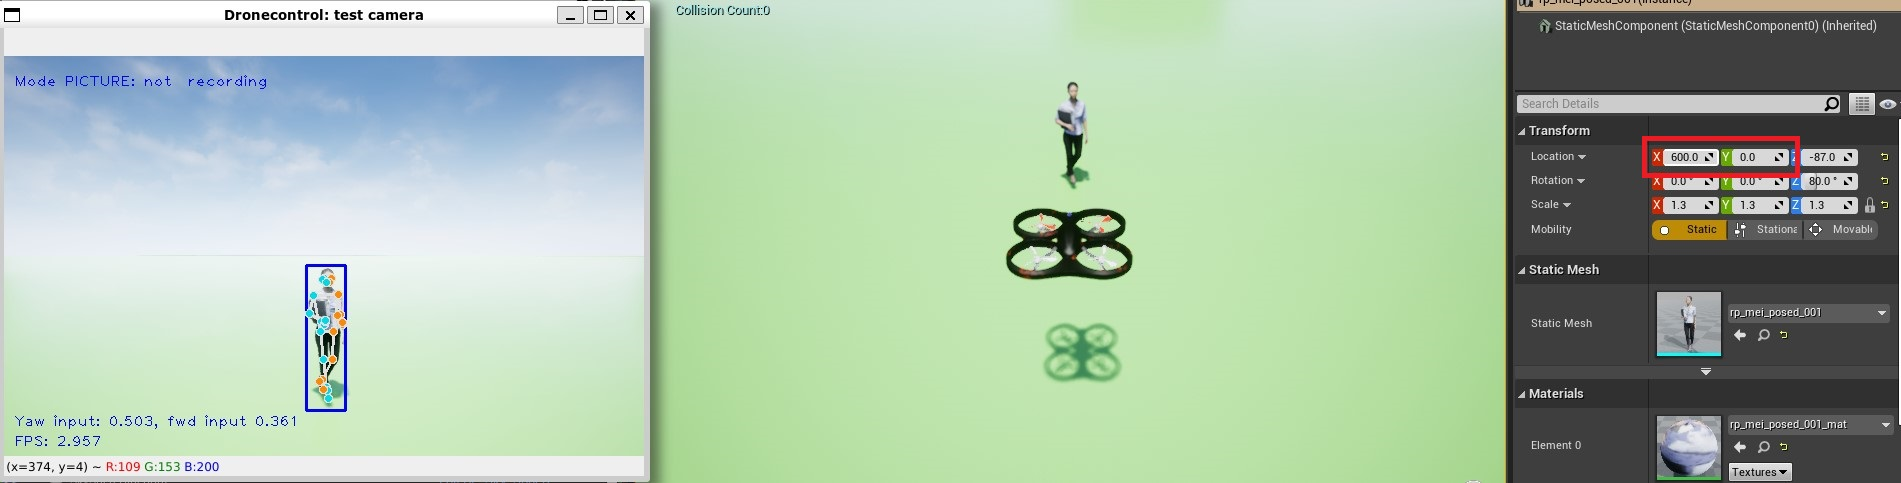
\includegraphics[width=\textwidth, keepaspectratio]{img/pid/tune-ref-pos.jpg}
  \caption{Reference position for the yaw and forward PID controllers. From left to right, the panels show the DroneVisionControl application window, the AirSim simulator world view and the world location of the human model in the simulator. The distance between the vehicle and the person is 600 units in the x direction and 0 units in the y direction.}
  \label{fig:tune-start-pos}
\end{figure}


\subsection{Yaw controller}

\begin{figure}
  \centering
  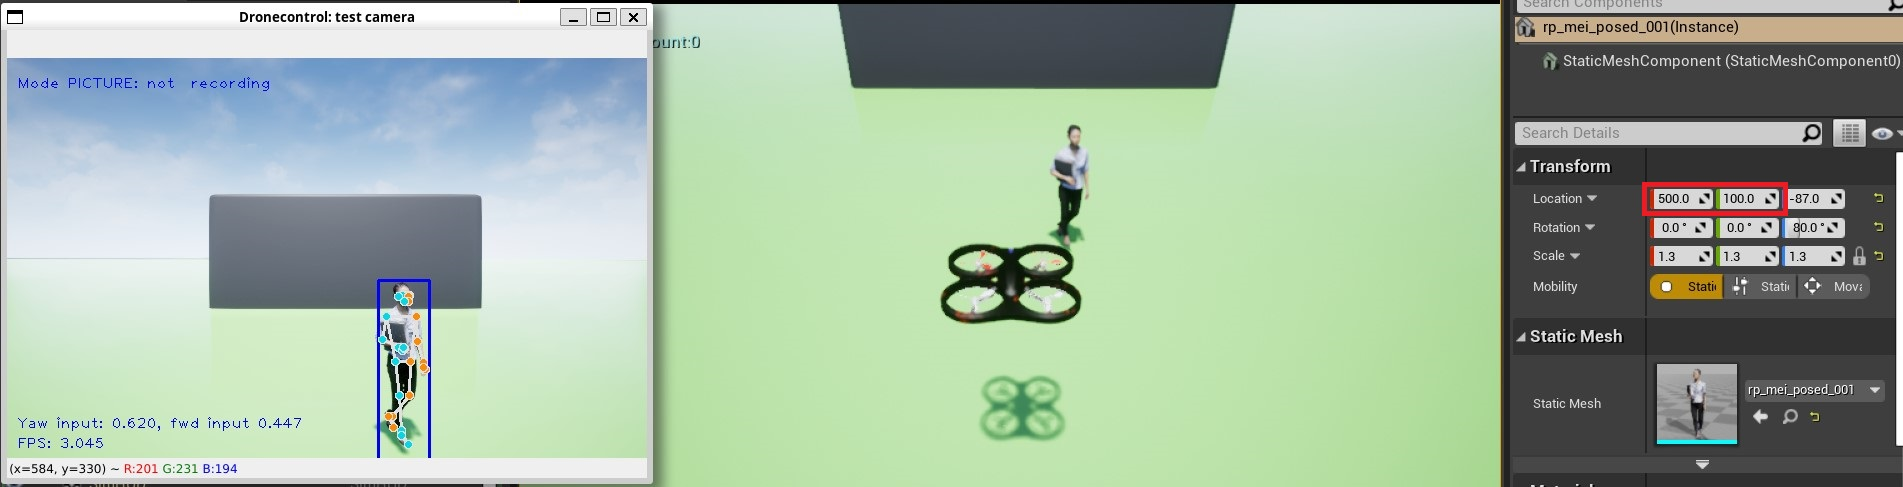
\includegraphics[width=\textwidth, keepaspectratio]{img/pid/tune-ref-pos-yaw.jpg}
  \caption{Starting position of the simulator for tuning the yaw controller. The human model is situated 500 units forward and 100 units to the right of the vehicle model.}
  \label{fig:tune-ref-pos-yaw}
\end{figure}

To find the correct coefficients for the controller that governs the yaw velocity of the vehicle, the target person is set in a position slightly to the side on its field of view so that when the controller is engaged, it outputs a rotation of the vehicle to that side.
Since the forward controller will not be engaged during the test, the target person can be situated closer to the camera to make it easier for the pose detection algorithm to output correct landmarks.
Figure \ref{fig:tune-ref-pos-yaw} shows the starting position of the simulated environment before each run, where the 3D model has been situated at (500, 100), that is, 100 units to the right of the reference position.
On the left-most panel of figure \ref{fig:tune-ref-pos-yaw}, the DroneVisionControl application shows that the input to the yaw controller is 0.62 at this position.
The controller must then output a positive yaw velocity to centre the person in its field of view. 
This offset position to the right produces an error that is less than zero (set point minus input, $\epsilon = 0.5 - 0.62$ ).
However, it requires a positive velocity to counteract and induce a yaw velocity to the right, so the coefficients for the yaw controller will need to be negative so that an increased horizontal position results in a positive yaw velocity to decrease it, as indicated by equation \ref{eq:pid}.
 

\begin{figure}
  \centering
  \makebox[\textwidth][c]{
  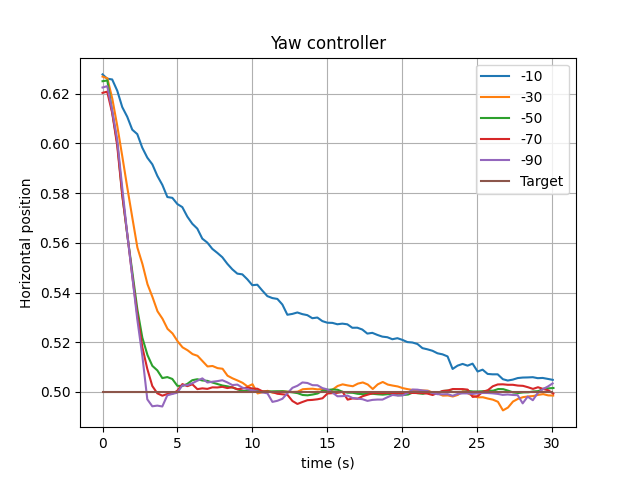
\includegraphics[width=.52\textwidth]{img/pid/yaw/yaw_pos_prop_i0_d0.png}
  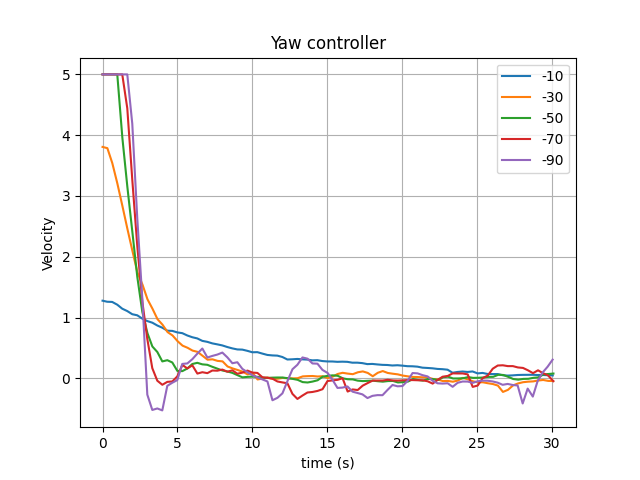
\includegraphics[width=.52\textwidth]{img/pid/yaw/yaw_vel_prop_i0_d0.png}}
  \caption{Variation of (a) input position and (b) output velocity for different values of $K_{P}$ and $K_I=0$, $K_D=0$ while the yaw controller is engaged.}\label{fig:tune-yaw-prop}
\end{figure}

To tune the controller to its correct coefficients, the first step will be to test different values of $K_{P}$ while maintaining $K_{I}$ and $K_{D}$ at zero.
Figure \ref{fig:tune-yaw-prop} shows the output of the tuning program for the five values of $K_{P}$ tested, from $K_P=-10$ to $K_P=-90$ in increments of 20.
The left graph represents the variation of the horizontal position detected by the camera for the first 30 seconds after activating the controller.
The right graph shows the yaw velocity that the controller outputs to the pilot module to reach the target.
For low values of $K_{P}$, the controller makes the vehicle move slowly towards its target so that it takes a long time to reach the midpoint position.
On the other hand, for high values of $K_{P}$, the controller tries to reach the target too fast, so when it gets close to it, it starts to oscillate around the target.
The right side graph also shows well how the output velocity in the yaw controller is limited to 5 degrees per second, so even for very high values of $K_P$, the vehicle will not rotate faster than that.
From the graphs, the best of the values tested is $K_{P}=50$, where the distance to the target point decreases rapidly (left graph), but the velocity does not start to increase and decrease widely around 0 (right graph).

The second step is to find the correct value for $K_I$. 
To do that, several values of $K_I$ will be tested for a low $K_P$ of -20 and $K_D=0$ so that the effect of the integral part is easier to appreciate. Figure \ref{fig:tune-yaw-int-20} shows the evolution of the input and output at the controller for a sample time of 40 seconds for each of the values tested. 
For a low $K_I=-1$, the progress toward the target is stable and slightly faster than without any contribution of the integral part.
However, when the $K_I$ increases in magnitude, it creates initial oscillations around the target position that fade out as time progresses. For a very large $K_I$ from around -10, the vehicle's velocity becomes locally unstable with many slight variations in its oscillations.

\begin{figure}
  \centering
  \makebox[\textwidth][c]{
  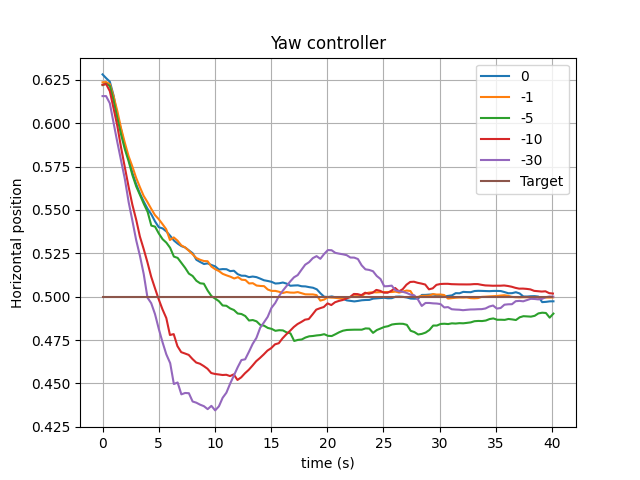
\includegraphics[width=.52\linewidth]{img/pid/yaw/yaw_pos_p20_int_d0.png}
  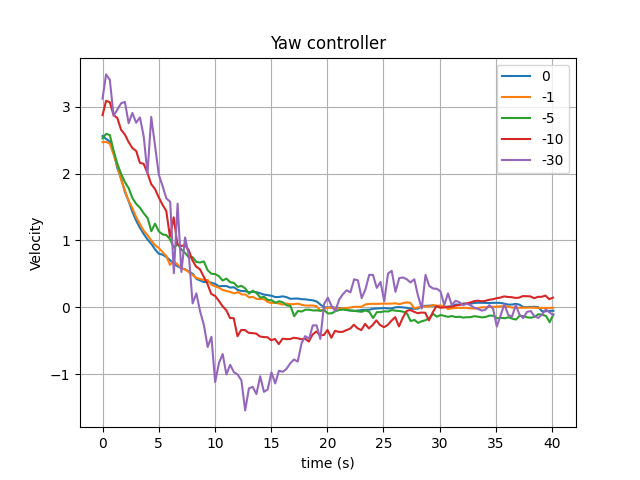
\includegraphics[width=.52\linewidth]{img/pid/yaw/yaw_vel_p20_int_d0.png}}
  \caption{Variation of (a) input position and (b) output velocity for different values of $K_{I}$ and $K_P=-20$, $K_D=0$ while the yaw controller is engaged.}\label{fig:tune-yaw-int-20}
\end{figure}

A similar effect can be observed to a lower extent in figure \ref{fig:tune-yaw-int-50}, where the measurements have been taken for $K_P=-50$ and $K_D=0$. 
In this graph, $K_I=-1$ makes the controller reach the target position some 3 seconds faster and with similar oscillations in its velocity than with the proportional part exclusively ($K_P=-50$, $K_I=0$, $K_D=0$).

\begin{figure}
  \centering
  \makebox[\textwidth][c]{
  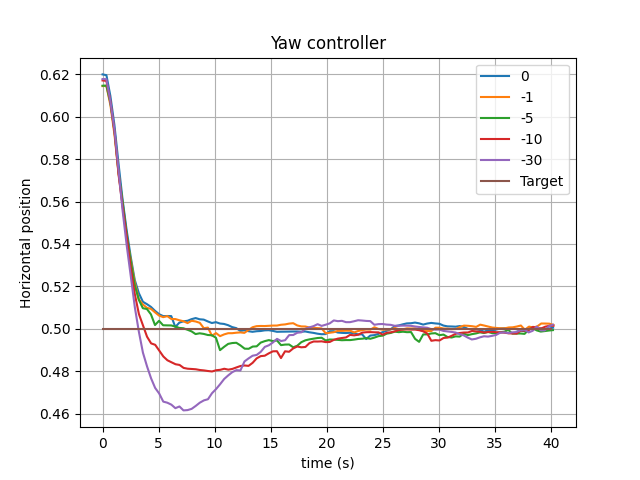
\includegraphics[width=.52\linewidth]{img/pid/yaw/yaw_pos_p50_int_d0.png}
  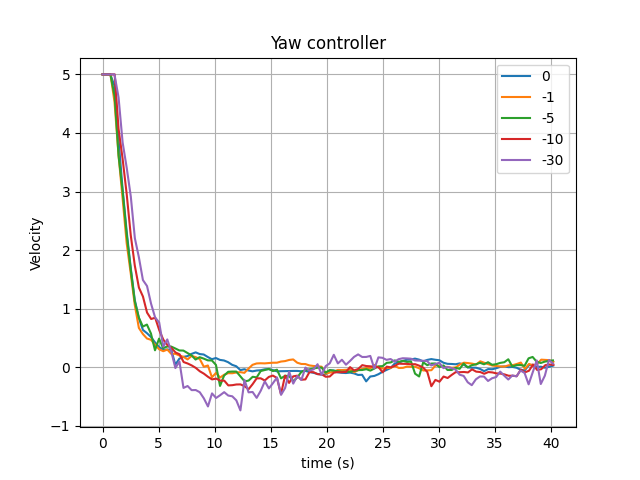
\includegraphics[width=.52\linewidth]{img/pid/yaw/yaw_vel_p50_int_d0.png}}
  \caption{Variation of (a) input position and (b) output velocity for different values of $K_{I}$ and $K_P=-50$, $K_D=0$ while the yaw controller is engaged.}\label{fig:tune-yaw-int-50}
\end{figure}

In the last step, the tuning process will deal with the derivative part of the controller.
In this case, several values of $K_D$ have been tested against the chosen $K_P=-50$, both without any integral part and with $K_I=-1$.
This will allow seeing the effect that the derivative part has in the controller, as well as validating if the integral part chosen in the last step can work together with the derivative part to make the controller react better to a changed input.
Figures \ref{fig:tune-yaw-der-i0} and \ref{fig:tune-yaw-der-i1} show the evolution of the position detected by the computer vision system and the velocity the controller outputs for a sample time of 40 seconds for $K_I=0$ and $K_I=-1$, respectively, with $K_P=-50$.
For all the tested values, the iteration with $K_I=-1$ on \ref{fig:tune-yaw-der-i1} shows a better convergence towards the target positions than their counterpart values of $K_D$ for $K_I=0$, which indicates that the integral part has been chosen correctly.
Furthermore, adding any amount to the derivative part does not produce any visible benefit in the step response of the controller and the curve that first stabilises on the target position continues to be the one for $K_D=0$, while the velocity graph remains approximately the same between $K_D=0$ and $K_D=-2$
The final values for the coefficients for the yaw controller will then be $K_P=-50$, $K_I=-1$, and $K_D=0$, so the controller will, in truth, only be a PI controller and not a complete PID controller.


\begin{figure}
  \centering
  \makebox[\textwidth][c]{
  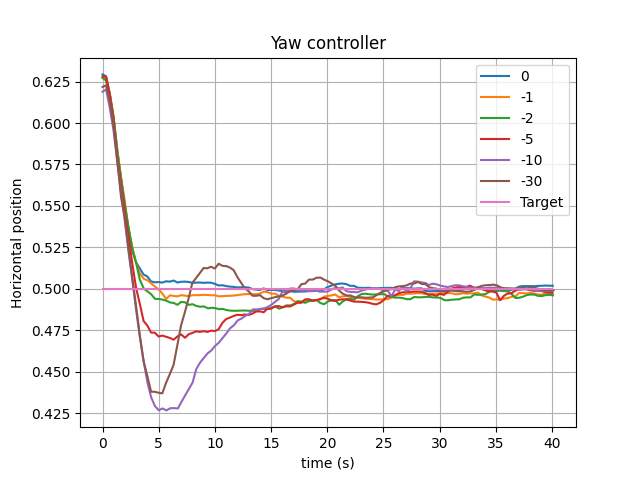
\includegraphics[width=.52\linewidth]{img/pid/yaw/yaw_pos_p50_i0_der.png}
  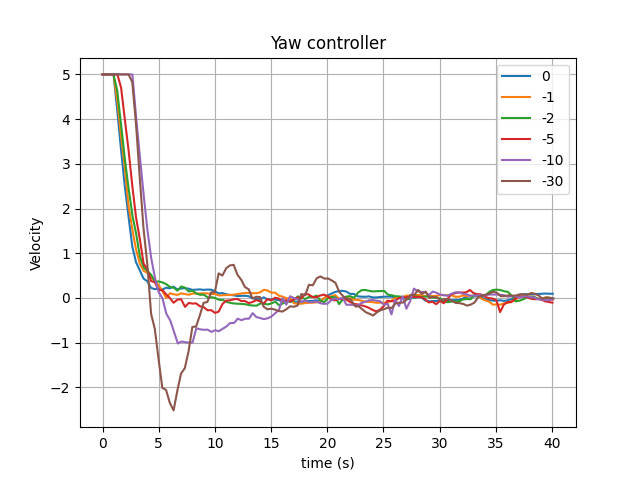
\includegraphics[width=.52\linewidth]{img/pid/yaw/yaw_vel_p50_i0_der.png}}
  \caption{Variation of (a) input position and (b) output velocity for different values of $K_{D}$ and $K_P=-50$, $K_I=0$ while the yaw controller is engaged.}\label{fig:tune-yaw-der-i0}
\end{figure}

\begin{figure}
  \centering
  \makebox[\textwidth][c]{
  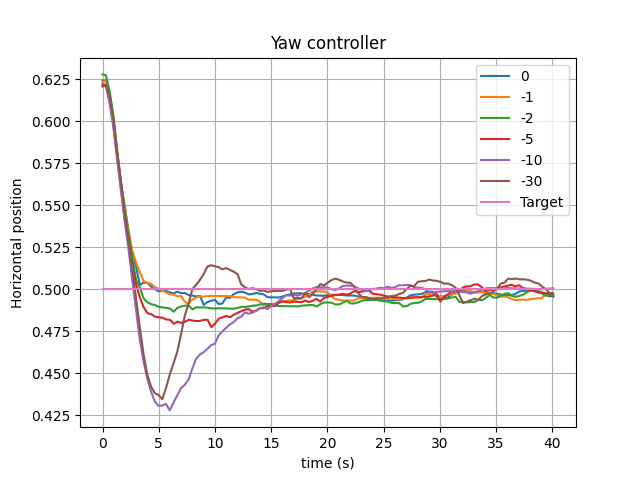
\includegraphics[width=.52\linewidth]{img/pid/yaw/yaw_pos_p50_i1_der.png}
  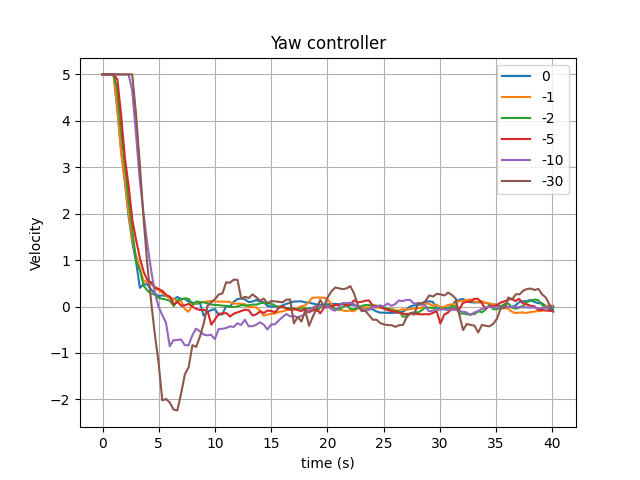
\includegraphics[width=.52\linewidth]{img/pid/yaw/yaw_vel_p50_i1_der.png}}
  \caption{Variation of (a) input position and (b) output velocity for different values of $K_{D}$ and $K_P=-50$, $K_I=-1$ while the yaw controller is engaged.}\label{fig:tune-yaw-der-i1}
\end{figure}

A recording of the whole tuning process for the yaw controller can be seen in this \href{https://l-gonz.github.io/tfg-giaa-dronecontrol/videos/tune-yaw-controller}{video}\footnote{\url{https://l-gonz.github.io/tfg-giaa-dronecontrol/videos/tune-yaw-controller}}.


\subsection{Forward controller}


A similar process to the one used for the yaw controller must be followed for the forward controller.
The starting position for the tuning process is, in this case, with the figure closer to the vehicle than the reference position and centred in its field of view.
Figure \ref{fig:tune-ref-pos-fwd} shows this starting setup with the figure situated at the (450,0) position in the simulated world.
In this position, the input to the forward controller is 0.47, that is, the bounding box around the detected figure takes up 47\% of the height of the camera field of view.
The response from the controller will therefore need to be a negative forward velocity that brings the vehicle away from the target person to reduce the perceived figure height.
Since a negative output velocity reduces the input at the entrance of the controller in a directly proportional manner, the coefficients for this PID controller will need to be positive, contrary to what happened on the yaw controller where the feedback loop was inversely proportional (a positive velocity decreased the input to the yaw controller).


\begin{figure}
  \centering
  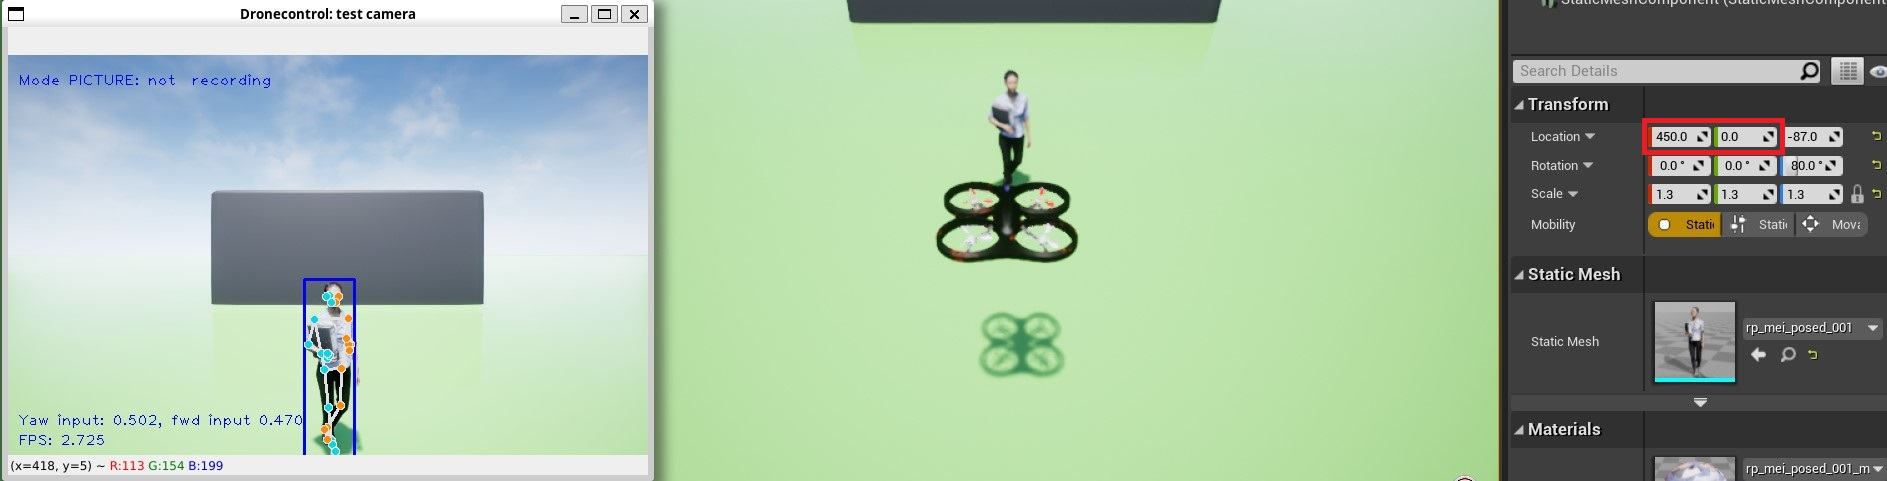
\includegraphics[width=\textwidth, keepaspectratio]{img/pid/tune-ref-pos-fwd.jpg}
  \caption{Starting position of the simulator for tuning the forward controller. The human model is situated 450 units forward and centred from the vehicle position.}\label{fig:tune-ref-pos-fwd}
\end{figure}

In general, the forward velocity will always need to be smaller than the yaw velocity since it induces a pitch angle in the vehicle that tilts the camera up and down, which can destabilise the camera and cause a loss of sight of the followed figure.
To achieve that, the coefficients for the forward controller will be reduced by one order of magnitude.
First, values from $K_P=1$ to $K_P=9$ in increments of 2 have been tested for $K_I=0$ and $K_D=0$ for a sample time of 30 seconds.
The curves described by the controller for these coefficients are shown in figure \ref{fig:tune-fwd-prop}.
Compared with the trajectory described by the yaw controller, the forward controller is generally more unstable since fast forward and backwards movements affect the pose detection algorithm.
This is particularly visible at the start of each test as slightly different heights are detected in the image from the camera even though the vehicle is in the same position with respect to the human figure.
It also creates an effect, especially for the bigger $K_P$ values tested, where, as the vehicle begins its movement back to its target position, the pose detection mechanism gets a slightly different perspective on the followed person, which increases the detected height slightly so that small spikes of detected differences show in the height graphs even though the velocity graph shows that the vehicle's direction of movement remains the same.
This effect is reduced by keeping the output forward velocity small in the controller.
In the right graph of figure \ref{fig:tune-fwd-prop}, it is also visible for high values of $K_P$ how the output velocity increases enough that the maximum velocity limit is reached on the forward controller and the output is capped to \unitfrac[0.4]{m}{s}.
For a value up to $K_P=3$, the trajectory described descends rapidly without ending in significant oscillations around the target height, so it is a fair value to keep for the final controller.


\begin{figure}
  \centering
  \makebox[\textwidth][c]{
  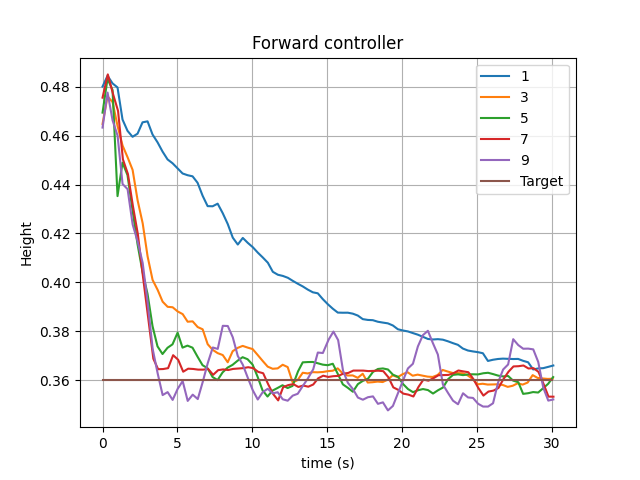
\includegraphics[width=.52\linewidth]{img/pid/fwd/aaa_fwd_pos_prop_i0_d0.png}
  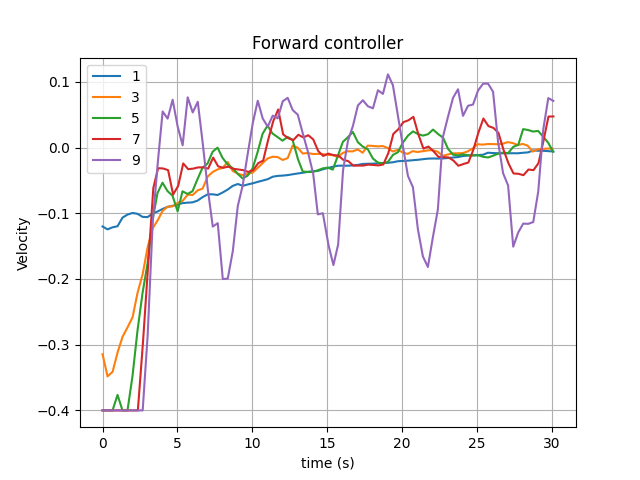
\includegraphics[width=.52\linewidth]{img/pid/fwd/aaa_fwd_vel_prop_i0_d0.png}}
  \caption{Variation of (a) input height and (b) output velocity for different values of $K_{P}$ and $K_I=0$, $K_D=0$ while the forward controller is engaged.}\label{fig:tune-fwd-prop}
\end{figure}


The respective tests for $K_I$ and $K_D$ in the forward controller are shown in figures \ref{fig:tune-fwd-int} and \ref{fig:tune-fwd-der}.
Increasing the coefficient for the integral part causes the controller to overshoot the target initially but then stabilise before starting to approximate to the target position.
Since, for this application, overshooting is not desirable, as it can cause safety issues, the chosen value of $K_I$ will be 0.
For the derivative part, every value of $K_D$ tested increases the system's oscillations, so it will also be left out of the forward controller.
The final values for the coefficients for the forward controller will then be $K_P=3$, $K_I=0$, and $K_D=0$, which makes it only a proportional controller.


\begin{figure}
  \centering
  \makebox[\textwidth][c]{
  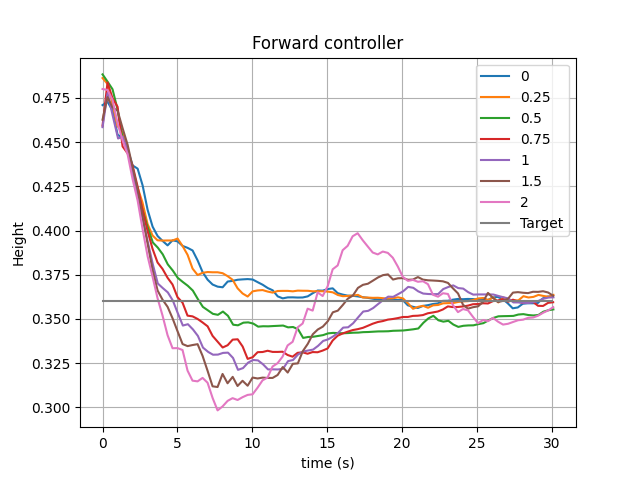
\includegraphics[width=.52\linewidth]{img/pid/fwd/aaa_fwd_pos_p3_int_d0.png}
  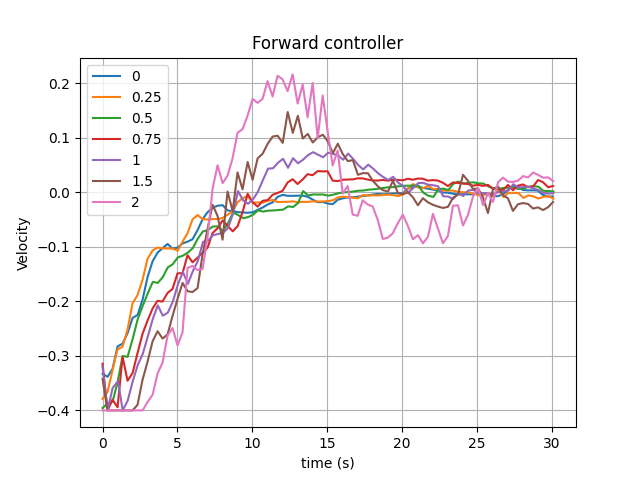
\includegraphics[width=.52\linewidth]{img/pid/fwd/aaa_fwd_vel_p3_int_d0.png}}
  \caption{Variation of (a) input height and (b) output velocity for different values of $K_{I}$ and $K_P=7$, $K_D=0$ while the forward controller is engaged.}\label{fig:tune-fwd-int}
\end{figure}
\begin{figure}
  \centering
  \makebox[\textwidth][c]{
  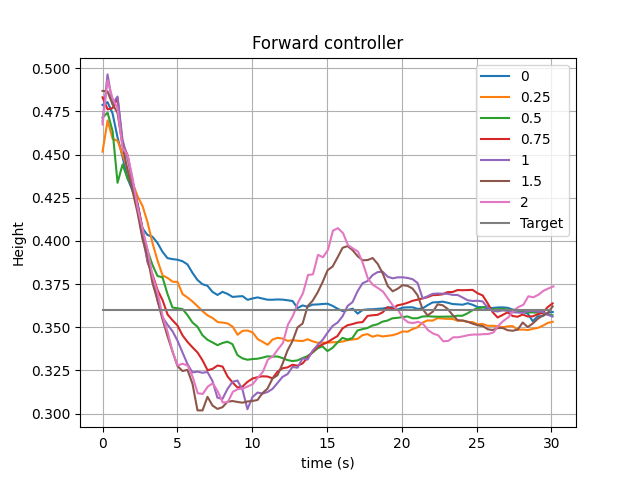
\includegraphics[width=.52\linewidth]{img/pid/fwd/aaa_fwd_pos_p3_i0_der.png}
  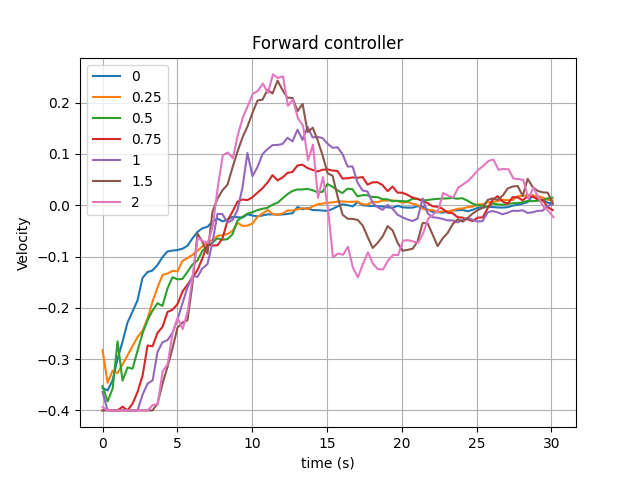
\includegraphics[width=.52\linewidth]{img/pid/fwd/aaa_fwd_vel_p3_i0_der.png}}
  \caption{Variation of (a) input height and (b) output velocity for different values of $K_{D}$ and $K_P=7$, $K_I=0.5$ while the forward controller is engaged.}\label{fig:tune-fwd-der}
\end{figure}


\subsection{PID tuning validation}
\label{subsec:pid-test-controller}

As a final validation for the tuning obtained previously, the \texttt{test-controller} tool described in section \ref{subsec:pid-tools} will be used to check the step response of the controllers to different starting distances for the same coefficients.
Additionally, for this test, both controllers will be engaged simultaneously to verify that they work well together.
Firstly, the positions will vary on the y-axis, that is, the figure will move from left to right in the field of view of the vehicle.
The values for the y coordinate to be tested will be between -150 and 150 units in increments of 50.
The x coordinate of the figure in the simulated world will remain at $x=500$.

Plots of the changes in normalised horizontal distance and normalised figure height detected by the person recognition algorithm during the time the vehicle takes to reach the target distance from the human figure for each of the tested positions can be seen in figure \ref{fig:validate-yaw}.
It is considered that the vehicle has reached its target when the error is less than 2\%, and the output speed at the controller is less than 10\% of the maximum value.
Furthermore, the whole testing process followed with the developed \texttt{test-controller} tool can be seen in this \href{https://l-gonz.github.io/tfg-giaa-dronecontrol/videos/test-yaw-controller}{video}\footnote{\url{https://l-gonz.github.io/tfg-giaa-dronecontrol/videos/test-yaw-controller}}.

Since each starting position differs in distance and orientation to the target, both controllers must be engaged to reach the centre.
The yaw controller then introduces a negative yaw velocity when the figure is on the left half of the camera's field of view and a positive yaw velocity when the figure is on the right half to reach the target horizontal distance of 0.5 (figure centred in the image received from the camera);
Moreover, the forward controller outputs a negative forward velocity to reduce the detected height of the figure from around 0.44 to the target 0.36 since the figure is 100 units closer to the vehicle than the reference position $x=600$.

Figure \ref{fig:validate-yaw}a shows that the most time is spent on starting the movement towards the target and, after that, there is not much difference between the time it takes to reach the -50 position and reaching the -150 position, with the former taking 3 seconds and the later taking around 3.6 seconds.
In figure \ref{fig:validate-yaw}b, all of the trajectories have a very similar graph since the starting distance to the target is practically the same, where the controller makes the vehicle pull backwards so the figure stays far enough, making the detected height decrease.
For the $y=100$ starting position, the initial detected height is very small in the beginning until it reaches the starting point of the other tests.
This occurred because the detection algorithm took longer than usual to identify the person in this particular test.
However, after less than half a second, the detection was stabilised without affecting much the time it took to reach the target or its final position, showing that the controllers can recover from errors in the detection mechanism without affecting the vehicle's movement.


\begin{figure}
  \centering
  \makebox[\textwidth][c]{
  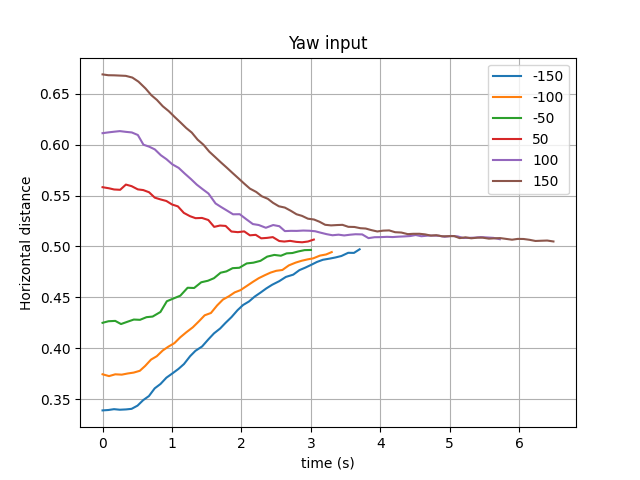
\includegraphics[width=.52\linewidth]{img/pid/validation_yaw.png}
  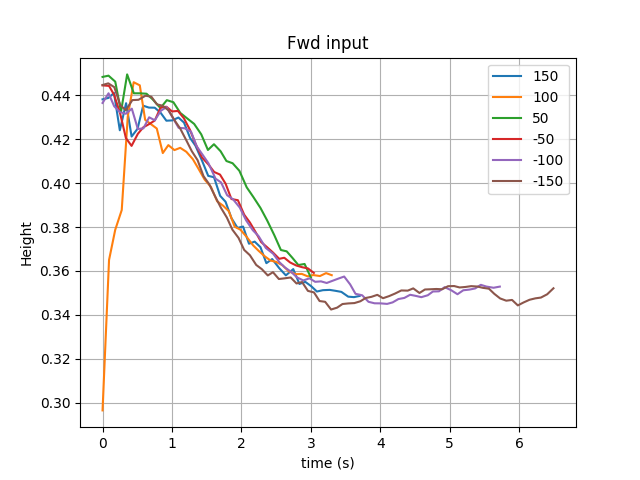
\includegraphics[width=.52\linewidth]{img/pid/validation_yaw_2.png}}
  \caption{Changes over time in detected horizontal position and height as input for the controllers with different starting positions in the y-axis}
  \label{fig:validate-yaw}
\end{figure}

Additionally, the \texttt{test-controller} tool can be run with varying positions in the x-axis, which means that the tests are run with the human figure at different distances closer and further away from the vehicle while maintaining it in the centre of its field of view (y position will remain 0 for the whole process).
Therefore, the yaw controller will not need to be considered for this test.
The changes over time in the input into the forward controller between each starting position and the target position are shown in figure \ref{fig:validate-fwd}.
The figure reflects a significant difference in how the controller reacts to positions closer than the target distance or further from it.
When the person is very close to the vehicle, there are major differences between detected heights, so the vehicle moves fast away from its position.
However, when the person is further away from the vehicle than the target, large differences in distance are associated with minor differences in detected height, which causes the controller to determine a smaller velocity increase than for the same distance difference if the person was closer to the vehicle.
Therefore it will take a longer amount of time for the vehicle to reach the target.
It is worth noting that even when the person is so close to the vehicle that part of it falls outside of its field of view ($x=300$ in the figure), the pose detection works well enough to interpret where the person should continue outside of the image so that it is still possible for the controller to decide the correct direction of movement.

\begin{figure}
  \centering
  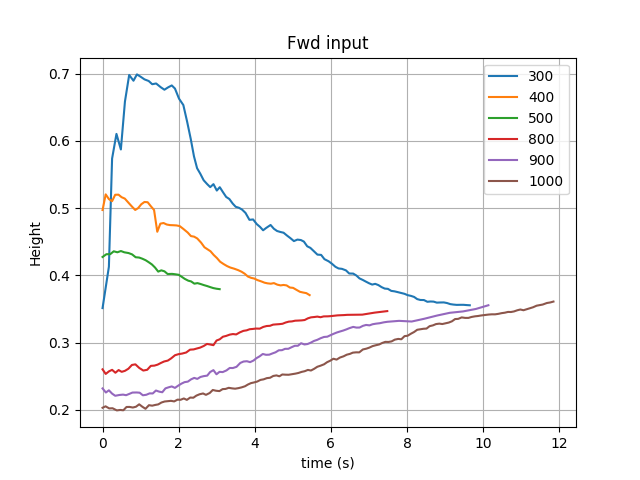
\includegraphics[width=.7\textwidth, keepaspectratio]{img/pid/validation_fwd.png}
  \caption{Changes over time in detected height as input for the forward controller with different starting positions in the x-axis}
  \label{fig:validate-fwd}
\end{figure}
